\documentclass[a4paper,11pt]{article}
\usepackage{amsmath,amsthm,amssymb}
\usepackage[utf8]{inputenc}
\usepackage[english,russian]{babel}
\usepackage[export]{adjustbox}
\usepackage{graphicx}
\usepackage{pgfplots}
\usepackage{textcomp}

\graphicspath{{pictures/}}
\DeclareGraphicsExtensions{.pdf,.png,.jpg}
\leftskip=-0cm 
\rightskip=-0cm
\voffset = -3cm
\hoffset = -3cm
\textwidth = 550pt
\textheight = 770pt
\pgfplotsset{width=10cm,compat=1.9}


\begin{document}
\Large
HW14
\\
1

\begin{center}
\center{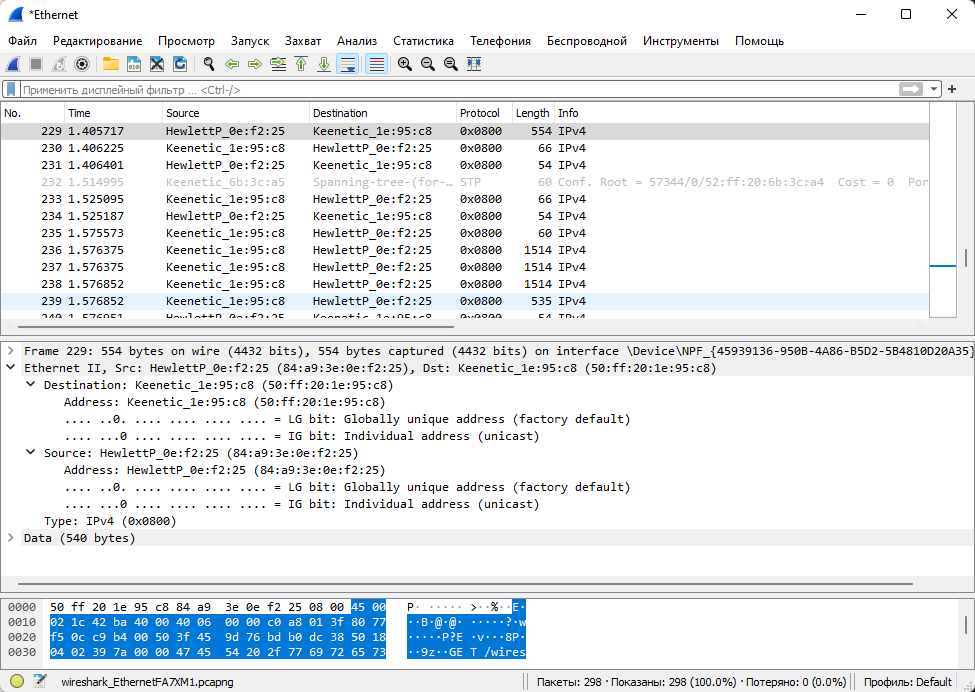
\includegraphics[width =\textwidth]{screenshots/1.png}}
\label{fig:image}
\end{center}
1) 84:a9:3e:0e:f2:25

2) HewlettP\_0e:f2:25

\begin{center}
\center{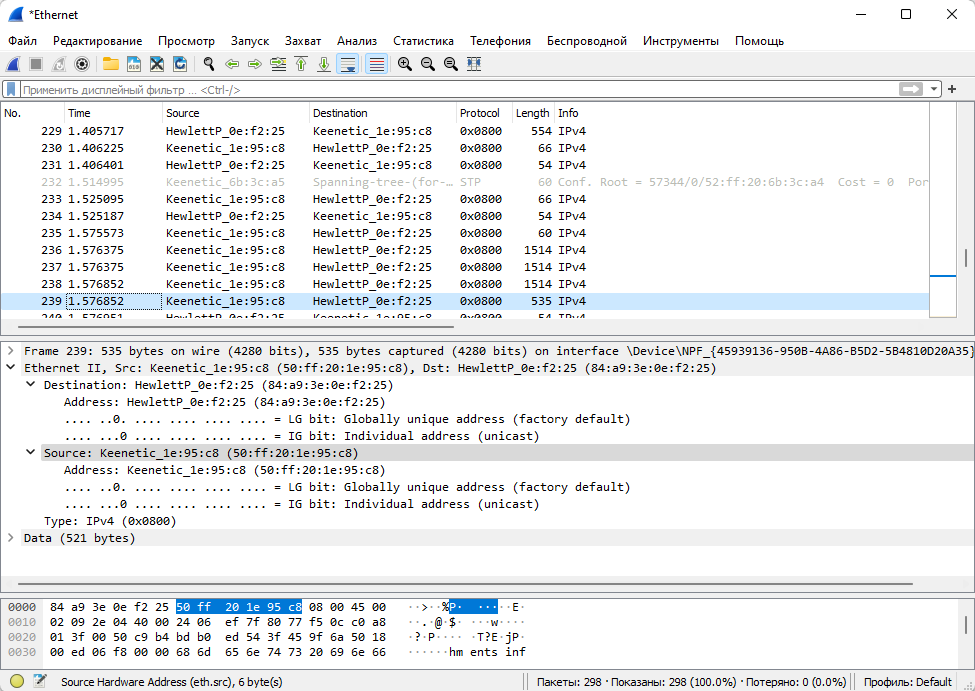
\includegraphics[width =\textwidth]{screenshots/2.png}}
\label{fig:image}
\end{center}
3) Source: Keenetic\_1e:95:c8 (50:ff:20:1e:95:c8) (в скобках адрес, до этого устройство)

4) Destination: HewlettP\_0e:f2:25 (84:a9:3e:0e:f2:25) (адрес моего компьютера)
\newpage
2

\begin{center}
\center{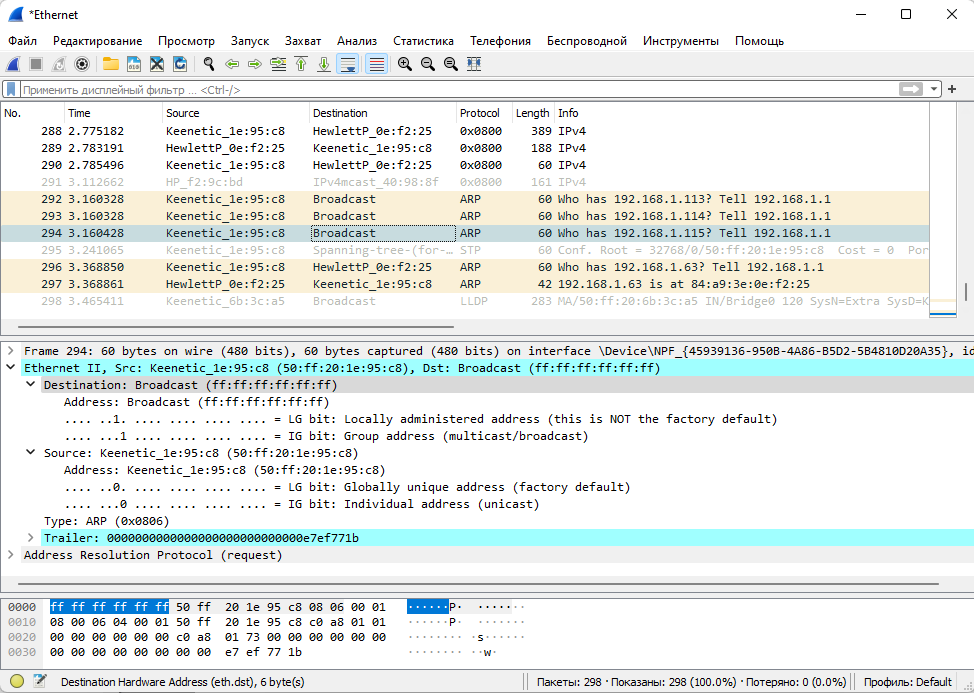
\includegraphics[width =\textwidth]{screenshots/3.png}}
\label{fig:image}
\end{center}
1) Src: 50:ff:20:1e:95:c8, Dst: ff:ff:ff:ff:ff:ff

\begin{center}
\center{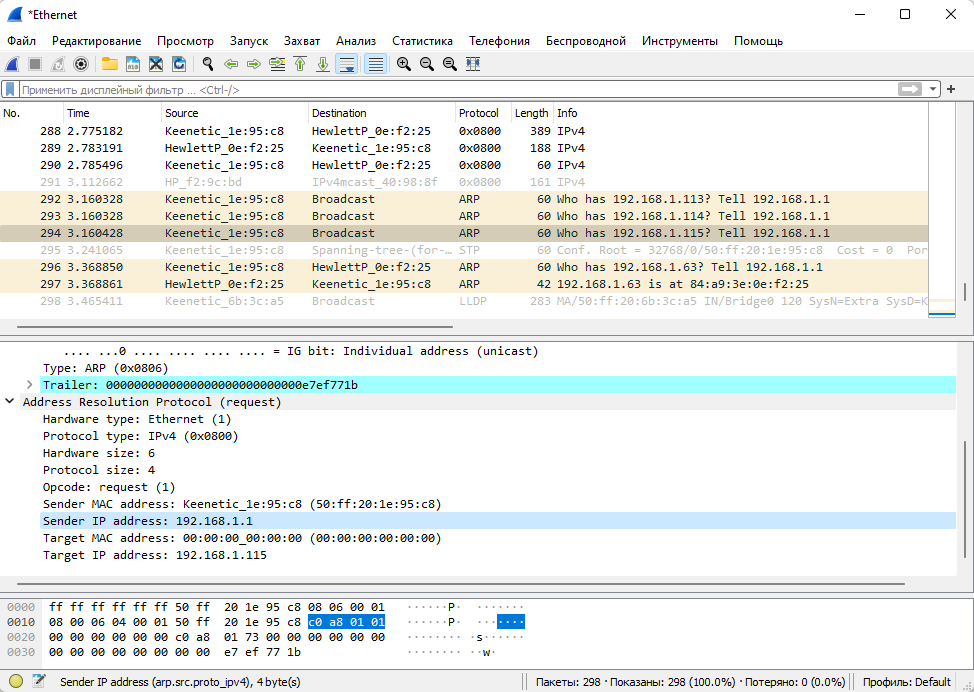
\includegraphics[width =\textwidth]{screenshots/4.png}}
\label{fig:image}
\end{center}
2) Sender IP address: 192.168.1.1

3) Target MAC address: 00:00:00\_00:00:00 (00:00:00:00:00:00) 

\begin{center}
\center{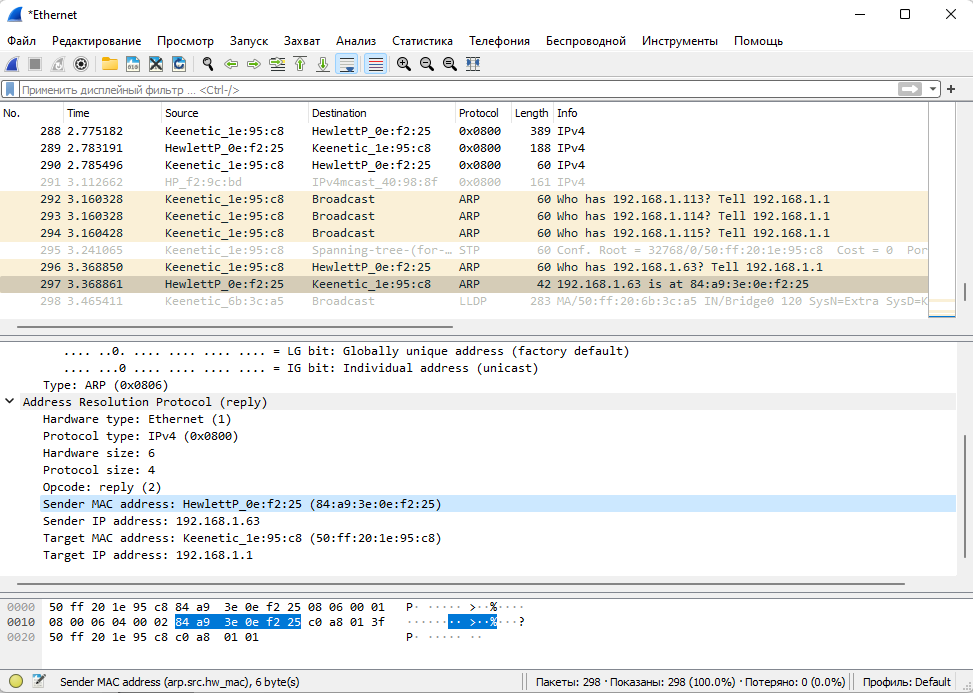
\includegraphics[width =\textwidth]{screenshots/5.png}}
\label{fig:image}
\end{center}
4) Sender MAC address: HewlettP\_0e:f2:25 (84:a9:3e:0e:f2:25)
\end{document}








































